\documentclass[11pt]{article}
\usepackage[a4paper,margin=1in]{geometry}
\usepackage{amsmath,amssymb,bm}
\usepackage{graphicx}

\title{Machine Learning Assignment 1}
\author{Zitian Wang}
\date{\today}

\begin{document}
\maketitle

\section{Problem 1: Ridge Regression}

We use the linear model $\hat y=\theta_0 + x^\top\theta$ with an \emph{unpenalized} intercept $\theta_0$.

\subsection*{(a) Objective (Ridge with unpenalized intercept)}
Given $\{(x_n,t_n)\}_{n=1}^N$, the ridge objective is
\[
J(\theta_0,\theta)
=\sum_{n=1}^N\bigl(t_n-\theta_0-x_n^\top\theta\bigr)^2
+\lambda\lVert\theta\rVert_2^2,\quad \lambda\ge 0.
\]
Let $\tilde X=[\,\mathbf 1,\ X\,]\in\mathbb R^{N\times(d+1)}$, $\tilde\theta=[\,\theta_0;\ \theta\,]$ and
$\Lambda=\mathrm{diag}(0,\lambda,\ldots,\lambda)$. Then
\[
J(\tilde\theta)=\lVert t-\tilde X\tilde\theta\rVert_2^2+\tilde\theta^\top\Lambda\,\tilde\theta.
\]

\subsection*{(b) MSE and closed-form solution}
The mean squared error is
\[
\mathrm{MSE}=\frac{1}{N}\sum_{n=1}^N\bigl(t_n-\theta_0-x_n^\top\theta\bigr)^2.
\]
Setting $\nabla J=0$ gives the normal equations
\[
\bigl(\tilde X^\top\tilde X+\Lambda\bigr)\tilde\theta=\tilde X^\top t
\quad\Rightarrow\quad
\boxed{\ \tilde\theta^\star=\bigl(\tilde X^\top\tilde X+\Lambda\bigr)^{-1}\tilde X^\top t\ }.
\]

\subsection*{(c) Effect of $\lambda$}
As $\lambda\to 0$, ridge $\to$ OLS (low bias, high variance). Larger $\lambda$ shrinks $\theta$ toward $0$ (higher bias, lower variance). The intercept $\theta_0$ is not penalized.

\subsection*{(d) Numeric example ($\lambda=0.8$)}
Data:
\[
X=\begin{bmatrix}
1&2\\2&1\\3&3\\4&2
\end{bmatrix},\quad
t=\begin{bmatrix}10\\12\\18\\21\end{bmatrix},\quad
\tilde X=\begin{bmatrix}
1&1&2\\1&2&1\\1&3&3\\1&4&2
\end{bmatrix},\quad
\Lambda=\mathrm{diag}(0,0.8,0.8).
\]
Compute
\[
\tilde X^\top\tilde X=\begin{bmatrix}4&10&8\\10&30&21\\8&21&18\end{bmatrix},\qquad
\tilde X^\top t=\begin{bmatrix}61\\172\\128\end{bmatrix}.
\]
Hence
\[
\tilde\theta^\star=
\begin{bmatrix}\theta_0^\star\\\theta_1^\star\\\theta_2^\star\end{bmatrix}
=
\bigl(\tilde X^\top\tilde X+\Lambda\bigr)^{-1}\tilde X^\top t
\approx
\begin{bmatrix}
5.2697\\[2pt]
3.1890\\[2pt]
1.0039
\end{bmatrix}.
\]

\paragraph{Check that $(\theta_0,\theta_1,\theta_2)=(1,2,1)$ is not optimal.}
Residual $r=t-\tilde X[1,2,1]^\top=[\,5,6,8,10\,]^\top$ gives
\[
\frac{\partial J}{\partial \theta_0}=-2\mathbf 1^\top r=-58\neq 0,\qquad
\frac{\partial J}{\partial \theta}=-2X^\top r+2\lambda\theta=\begin{bmatrix}-158.8\\-118.4\end{bmatrix}\neq\bm 0.
\]
So first-order optimality fails.

\paragraph{Error comparison (MSE).}
\[
\mathrm{MSE}(1,2,1)=56.25,\qquad
\mathrm{MSE}(\tilde\theta^\star)=0.3998.
\]
(With the ridge objective $J=\mathrm{SSE}+\lambda\|\theta\|^2$: $J(1,2,1)=229.0$ and $J(\tilde\theta^\star)=10.5413$.)
\section{Problem 2: Kernel Methods}

\subsection*{(a) What are kernel methods?}
Kernel methods map inputs via a (possibly infinite\!-)dimensional feature map $\phi:\mathbb{R}^d\!\to\!\mathcal{H}$ and then apply a \emph{linear} algorithm in $\mathcal{H}$. The \emph{kernel trick} evaluates inner products by a kernel
$k(x,y)=\langle\phi(x),\phi(y)\rangle$
without forming $\phi(x)$ explicitly, enabling nonlinear decision boundaries in the original input space.

\subsection*{(b) Is $k(x,y)=(x^\top y)^d$ a valid kernel?}
Yes. Define the $d$-fold tensor feature map $\phi(x)=x^{\otimes d}\in\mathbb{R}^{d^d}$ (or, equivalently, the vector of all degree-$d$ monomials, up to a fixed scaling). Then
\[
\langle \phi(x),\phi(y)\rangle
=\langle x^{\otimes d},\,y^{\otimes d}\rangle
=(x^\top y)^d,
\]
so the corresponding Gram matrix is symmetric positive semidefinite. Hence $(x^\top y)^d$ is a valid (homogeneous polynomial) kernel.

\subsection*{(c) Memory cost: linear vs.\ kernel ridge}
\begin{itemize}
  \item \textbf{Linear ridge:} store $X\in\mathbb{R}^{N\times d}$ and (optionally) $X^\top X\in\mathbb{R}^{d\times d}$.
        Memory $\mathcal{O}(Nd)+\mathcal{O}(d^2)$.
  \item \textbf{Kernel ridge:} form the Gram matrix $K\in\mathbb{R}^{N\times N}$ and solve $(K+\lambda I)\alpha=t$.
        Memory $\mathcal{O}(N^2)$.
\end{itemize}
Thus, kernel methods become memory–heavy when $N$ is large, while linear methods scale better with $N$ (but may require large $d$).
\section{Problem 3: Support Vector Machines}

\subsection*{(a) Linear separability}
From the scatter of the given 2D points, the two classes are linearly separable.
\begin{figure}[h]
    \centering
    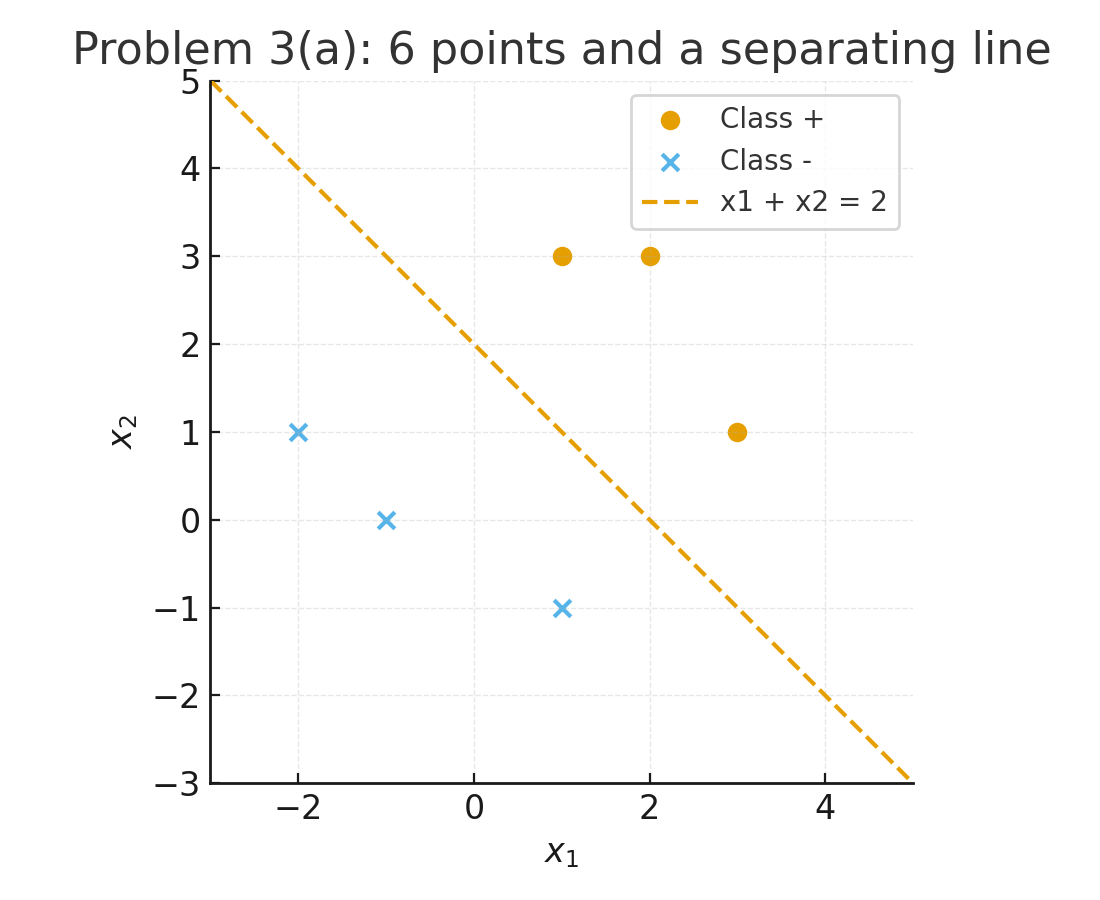
\includegraphics[width=0.65\linewidth]{./problem3a_svm_plot_fixed.png}
    \caption{Problem 3(a): 2D points and a separating line $x_1+x_2=2$.}
  \end{figure}
  
\subsection*{(b) Maximum-margin separator}
A maximum-margin separator is
\[
x_1 + x_2 = 2
\quad\Longleftrightarrow\quad
w=\begin{bmatrix}1\\[2pt]1\end{bmatrix},\ b=-2.
\]
In canonical SVM scaling (i.e., $y_i(w^\top x_i+b)\ge 1$), take
\[
w'=\tfrac12\!\begin{bmatrix}1\\[2pt]1\end{bmatrix},\quad b'=-1.
\]
Then the support vectors satisfy equality:
\[
\text{SV (+)}:\ (3,1),(1,3);\qquad \text{SV (–)}:\ (1,-1),
\]
since $w'^\top(3,1)+b'=\tfrac12(4)-1=1$, $w'^\top(1,3)+b'=1$, and $w'^\top(1,-1)+b'=-1$.

\subsection*{(c) Margin width}
With the canonical scaling, the margin width is
\[
\gamma \;=\; \frac{2}{\|w'\|_2}
\;=\; \frac{2}{\sqrt{(1/2)^2+(1/2)^2}}
\;=\; 2\sqrt{2}.
\]

\subsection*{(d) Using a quadratic kernel}
Using a degree-2 polynomial kernel maps points to a higher-dimensional feature space where the data are also separable. The maximum margin is computed in that feature space and generally differs (and is not directly comparable in value) to the geometric margin measured in the original input space. Since the data are already linearly separable, a kernel does not improve separability per se, though it changes the geometry of the optimization.

\subsection*{(e) Adding $(2,0.5)$ labeled as ``+''}
Under the separator in (b), the functional margin is
\[
f(2,0.5)=w'^\top(2,0.5)+b'=\tfrac12(2+0.5)-1=0.25>0,
\]
so it is still classified as ``+'' but lies \emph{inside} the margin band ($|f|<1$). Hence the old hard-margin solution is no longer feasible for the augmented dataset. In a soft-margin SVM, this point incurs slack
\[
\xi=\max\{0,\,1 - y f(x)\}=1-0.25=0.75,
\]
trading off margin violation against the hinge-loss penalty.

\end{document}
